
\documentclass[12pt]{report}
\usepackage{geometry}
\geometry{a4paper}
\usepackage{chicago}
\usepackage{makeidx}
\usepackage{tabularx}
\usepackage{graphicx}
\usepackage{color}
\usepackage{pdfpages}

\def\keywords{\vspace{.5em}
{\textbf{Keywords} \linebreak \,\relax%
}}
\def\endkeywords{\par}


\begin{document}
\begin{titlepage}
\begin{center}

% Upper part of the page. The '~' is needed because \\
% only works if a paragraph has started.
\textbf{\LARGE The University of Birmingham}\\[0.35cm]
\textbf{\LARGE School of Computer Science}\\[0.35cm]
\textbf{\LARGE MSc in Advanced Computer Science}\\[2.5cm]

\textsc{\Large Second semester mini-project}\\[2.5cm]

% Title

{ \huge \bfseries  Analysing User Interaction On Mobile Devices \\[1cm] }

{\large \textbf{Karthikeya Udupa Kuppar Manjunath}\\[1cm]}

\large{Supervisor: Mirco Musolesi}
% Author and supervisor


\vfill

% Bottom of the page
{\large April 2014}

\end{center}
\end{titlepage}

\begin{abstract}

abstract here.
\linebreak\linebreak\linebreak\linebreak
\begin{center}
\begin{keywords}
keywords here.
\end{keywords}
\end{center}
\end{abstract}


\tableofcontents
\listoffigures
\listoftables
\newpage

\chapter{Introduction}
\noindent
Over the last two decades the world has been revolutionised by technologies beyond what could have been even imagined a century ago. The digital revolution has effected our lives in every possible aspect, mobility is one of the key components of this revolution and has been incorporated in people's live at a very drastic rate [14 -1]. Smart phones and portable devices have become an extension of our persona and have been personalised by us, they reflect our preferences, social choices we make, places we go even the food we prefer to eat. These devices have provided a new meaning to the vision of Mark Wesiser [1] and also a means to achieve more with the network of wireless sensors in the hands of the people providing realtime information [7]. As we can see in section [x], much work has been done in this direction to make the vision a reality, systems that can provide a groundwork to build ubiquitous systems, algorithms to process the data and make inferences have been developed. This is what we are trying to accomplish in our research as well.

A key component of creating a building block for such a ubiquitous and anticipatory system would be to understand why people perform the actions that they perform at the given time [13] and how it be generalised across the masses which would eventually helps improves their lives without and not be a hindrance, anticipating their actions and adapt itself to their needs [12], Tennehouse [12-43] introduces this concept as proactive computing wherein the system would become so familiar with the user that it would be able to perform action on user's behest.

For us to accomplish this we would need a way in which we can monitor what activities people perform, what are the various contexts which effect these actions and to be able to do this on a large scale. Demographics have been proven to be a very important aspect in extracting features of the user as an individual [12, 4] and also as a collective [6, 3].

This whole process involves a lot of complexities surrounding it, firstly there is an issue of a platform to target, there is also a concern that in achieving such a system we might end up violating user's privacy and interfere in his life all of which among many other are once we address in this research.

\section{Context}
To understand what are the various circumstances under which the user takes a particular action on the device we analyse the \textit{Context} in which the user reacted in the given way. Context
\section{Anticipatory System}
\chapter{Context Sensing Framework}
\chapter{User Demographics Data Collection Application}
\chapter{Research Value of Data Collected}
\chapter{Performance Evaluation}
\chapter{Negative Aspects}    
\chapter{Related Work}
\chapter{Future Work}
\chapter{Conclusion}

\bibliographystyle{ abbrv}
\bibliography{mini_project_report}

%APPENDICES
\appendix
%Mini-project declaration
%\clearpage
\chapter{Mini-Project Declaration}
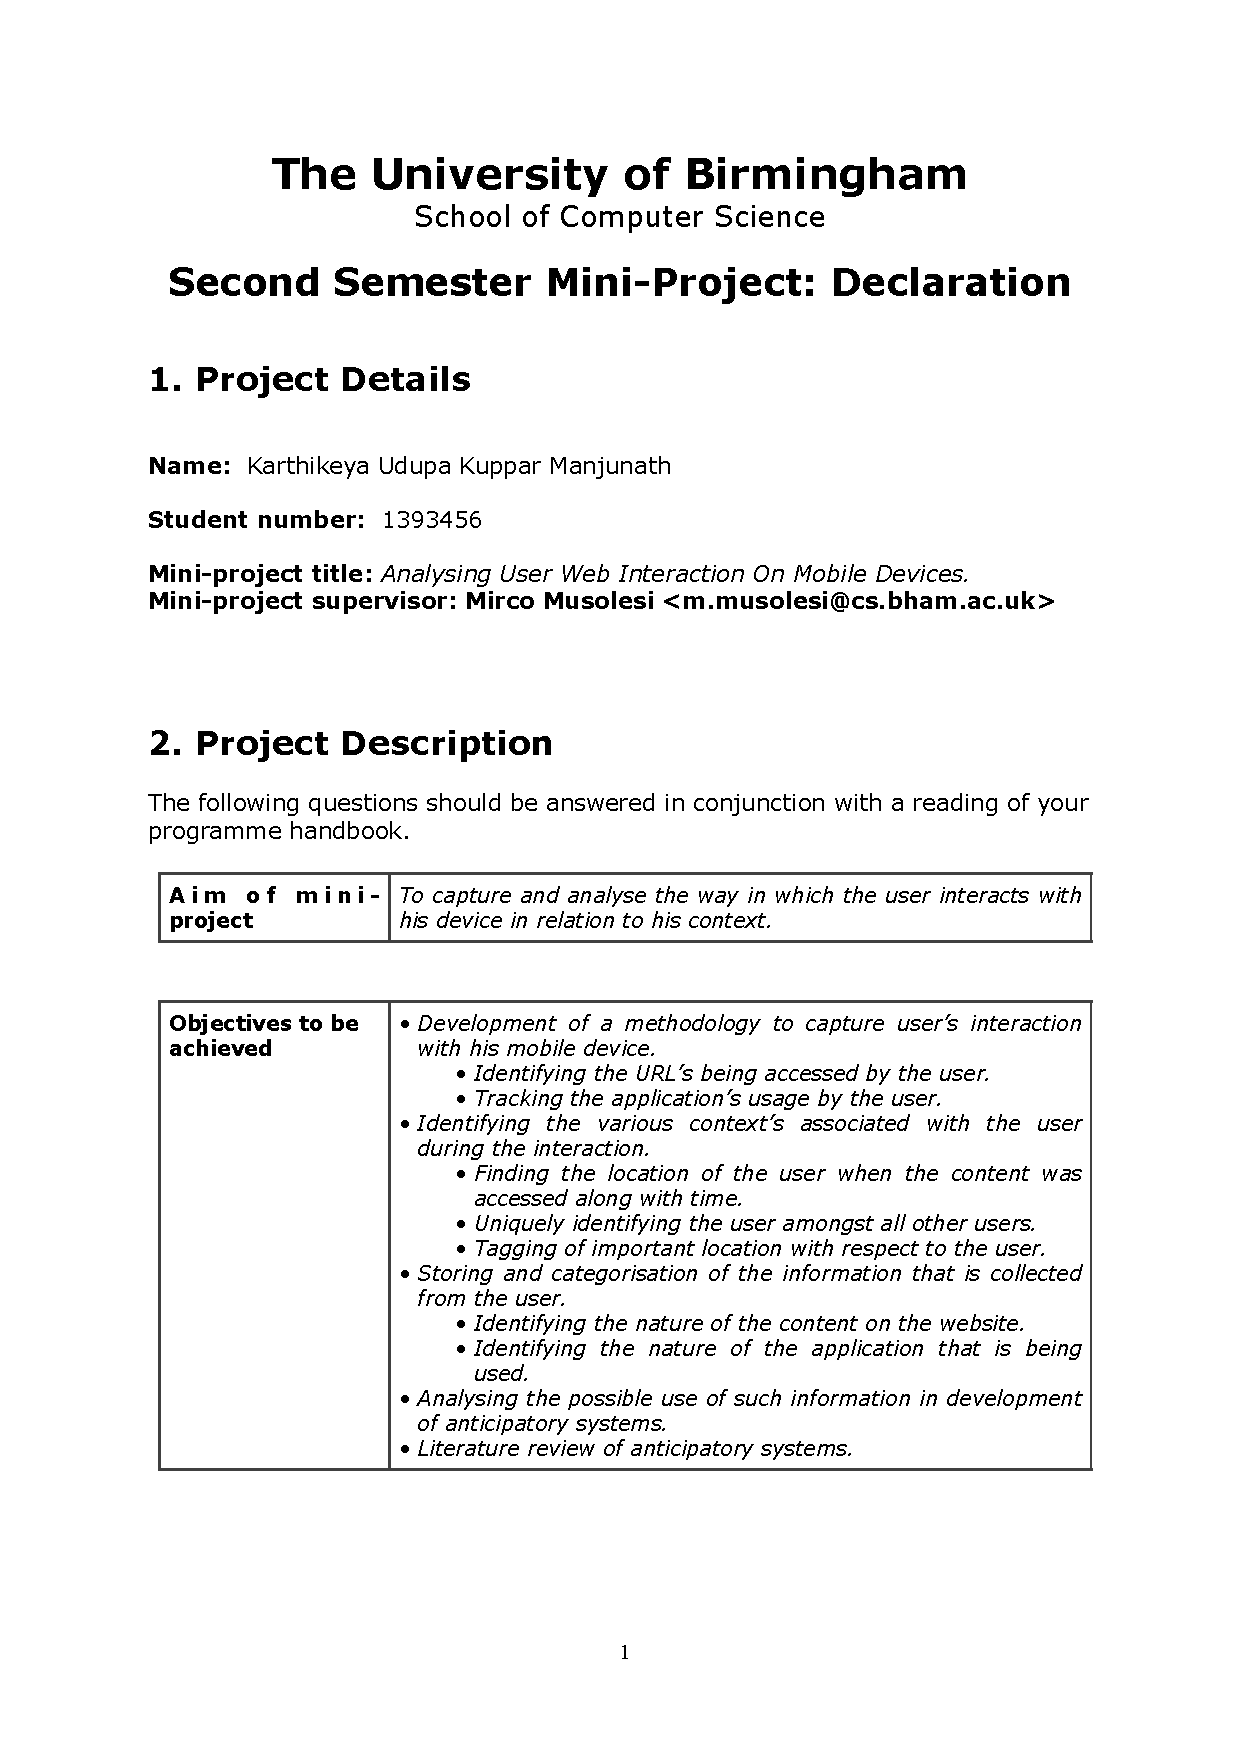
\includepdf[pages={1,2}]{Declaration.pdf}

\chapter{Statement of information search strategy}

statement of search
\end{document}